\documentclass{article}
\usepackage{IJCGA,algorithm,algorithmic,amsfonts}
\usepackage{latexsym}
\usepackage{psfig}
\usepackage{graphicx}
\usepackage{ipe}
\usepackage{url}
%\myheader{Improved Subdivision Traversal}

\newlength{\graphheight}
\setlength{\graphheight}{3in}

\newcommand{\centerpsfig}[1]{\centerline{\psfig{#1}}}

\newcommand{\centeripe}[1]{\begin{center}\Ipe{#1}\end{center}}

\newcommand{\seclabel}[1]{\label{sec:#1}}
\newcommand{\Secref}[1]{Section~\ref{sec:#1}}
\newcommand{\secref}[1]{\mbox{Section~\ref{sec:#1}}}

\newcommand{\alglabel}[1]{\label{alg:#1}}
\newcommand{\Algref}[1]{Algorithm~\ref{alg:#1}}
\newcommand{\algref}[1]{\mbox{Algorithm~\ref{alg:#1}}}

\newcommand{\applabel}[1]{\label{app:#1}}
\newcommand{\Appref}[1]{Appendix~\ref{app:#1}}
\newcommand{\appref}[1]{\mbox{Appendix~\ref{app:#1}}}

\newcommand{\tablabel}[1]{\label{tab:#1}}
\newcommand{\Tabref}[1]{Table~\ref{tab:#1}}
\newcommand{\tabref}[1]{Table~\ref{tab:#1}}

\newcommand{\figlabel}[1]{\label{fig:#1}}
\newcommand{\Figref}[1]{Figure~\ref{fig:#1}}
\newcommand{\figref}[1]{\mbox{Figure~\ref{fig:#1}}}

\newcommand{\eqlabel}[1]{\label{eq:#1}}
\newcommand{\eqref}[1]{(\ref{eq:#1})}

\newtheorem{thm}{Theorem}{\bfseries}{\itshape}
\newcommand{\thmlabel}[1]{\label{thm:#1}}
\newcommand{\thmref}[1]{Theorem~\ref{thm:#1}}

\newtheorem{lem}{Lemma}{\bfseries}{\itshape}
\newcommand{\lemlabel}[1]{\label{xlem:#1}}
\newcommand{\lemref}[1]{Lemma~\ref{xlem:#1}}

\newtheorem{cor}{Corollary}{\bfseries}{\itshape}
\newcommand{\corlabel}[1]{\label{cor:#1}}
\newcommand{\corref}[1]{Corollary~\ref{cor:#1}}

\newtheorem{obs}{Observation}{\bfseries}{\itshape}
\newcommand{\obslabel}[1]{\label{obs:#1}}
\newcommand{\obsref}[1]{Observation~\ref{obs:#1}}

%\newtheorem{assumption}{Assumption}{\bfseries}{\rm}
\newenvironment{ass}{\begin{assumption}\rm}{\end{assumption}}
\newcommand{\asslabel}[1]{\label{ass:#1}}
\newcommand{\assref}[1]{Assumption~\ref{ass:#1}}

\newcommand{\proclabel}[1]{\label{alg:#1}}
\newcommand{\procref}[1]{Procedure~\ref{alg:#1}}

\newcommand{\dist}{\mathit{dist}}


\newcommand{\rev}{\mathit{rev}}
\newcommand{\scc}{\mathit{succ}}
\newcommand{\pt}{\mathit{pt}}
\newcommand{\cwangle}{\stackrel{\mathrm{cw}}{\angle}}
\newcommand{\ccwangle}{\stackrel{\mathrm{ccw}}{\angle}}
\newcommand{\val}{\mathit{key}}
\newcommand{\entry}{\mathit{entry}}
\newcommand{\parent}{\mathit{parent}}
\newcommand{\src}{\mathit{src}}
\newcommand{\tgt}{\mathit{tgt}}
\newcommand{\minval}{\mathit{minval}}
\newcommand{\prd}{\mathit{pred}}
\newcommand{\rightturn}{\mathit{right\_turn}}
\newcommand{\face}{\mathit{face\_of}}
\newcommand{\cone}{\mathit{cone}}

\newcommand{\bkoo}{\textsc{bkoo}}
\newcommand{\bosemorin}{\textsc{bm}}
\newcommand{\dfs}{\textsc{dfs}}

\newcommand{\key}{\mathit{key}}

\newcommand{\etal}{\emph{et al}}

\newcommand{\return}{\textbf{return}}
\newcommand{\report}{\textbf{report}}


\title{\MakeUppercase{An Improved Algorithm for Subdivision Traversal 
	without Extra Storage}%
	\thanks{This research was funded by the Natural Sciences and 
	Engineering Research Council of Canada.}}

\author{\MakeUppercase{Prosenjit Bose} and \MakeUppercase{Pat Morin}\\[2pt]
	\textit{School of Computer Science, 
		Carleton University, 1125 Colonel By Drive \\ 
	Ottawa, Ontario, K1S 5B6, Canada \\
	\{jit,morin\}@cs.carleton.ca}}
\date{}{}

\begin{document}

\copyrightheading

% This produces an error
%\symbolfootnote
% so I use this instead
\renewcommand{\thefootnote}{\fnsymbol{footnote}}


\textlineskip

\begin{center}
\cgatitle{\MakeUppercase{An Improved Algorithm for Subdivision Traversal 
	without Extra Storage}%
	\footnote{This research was funded by the Natural Sciences and 
	Engineering Research Council of Canada.}}

\vspace{24pt}

{\authorfont \MakeUppercase{Prosenjit Bose} and 
	\MakeUppercase{Pat Morin}}

\vspace{2pt}

\addressfont{School of Computer Science, Carleton University \\
	1125 Colonel By Drive, Ottawa, Ontario, K1S 5B6, Canada}

\vspace{20pt}
%% authors need not care about this
\publisher{(received date)}{(revised date)}{Editor's name}

\end{center}

\alphfootnote

\begin{abstract}
We describe an algorithm for enumerating all vertices, edges and faces
of a planar subdivision stored in any of the usual pointer-based
representations, while using only a constant amount of memory beyond
that required to store the subdivision.  The algorithm is a refinement
of a method introduced by \mbox{de Berg} \etal\ (1997), that reduces
the worst case running time from $O(n^2)$ to $O(n\log n)$. We also
give experimental results that show that our modified algorithm runs
faster not only in the worst case, but also in many realistic cases.
\keywords{computational geometry, vertex enumeration, subdivision traversal, geographic information systems}
\end{abstract}

%%%%%%%%%%%%%%%%%%%%%%%%%%%%%%%%%%%%%%%%%%%%%%%%%%%%%%%%%%%%%%%%%%%%%%%%%
\textlineskip
\section{Introduction}

A planar subdivision $S$ is a partitioning of the plane into a set $V$
of vertices (points), a set $E$ of edges (line segments), and a set
$F$ of faces (polygons).  Planar subdivisions are frequently used in
geographic information systems as a representation for maps.  A common
operation on subdivisions is that of traversal.  Traversing a
subdivision involves reporting each vertex, edge and face of $S$
exactly once, so that, e.g., some operation can be applied to each.

The usual method of traversing a subdivision involves a breadth-first
or depth-first traversal of the primal (vertices and edges) or dual
(faces and edges) graph of $S$.  Unfortunately, this requires the use
of mark bits on the edges, vertices, or faces of $S$ and a stack or
queue.  If the data structure used to represent $S$ does not have
extra memory allocated to the vertex/edge/face records for these mark
bits, then an auxiliary array must be allocated and some form of
hashing is required to map vertex/edge/face records to array indices.
Even if extra memory is available for mark bits, this approach has the
problem that traversal cannot be done simultaneously by more than one
thread of execution without some type of locking mechanism.

For these reasons, researchers have investigated methods of traversing
subdivisions and other graph-like data structures without the use of
mark bits.\cite{bkoo97,egs86,gc86,gcr77,gm78}  Generally speaking,
these techniques use geometric properties of $S$ to define a spanning
tree $T$ of the vertices, edges or faces of $S$ and then apply a
well-known tree-traversal technique to traverse $T$ using $O(1)$
additional memory.

The most recent and general result on traversing planar subdivisions
is that of \mbox{de Berg} \etal\cite{bkoo97} who show how to
traverse any connected subdivision $S$ using only $O(1)$ additional
storage.  The running time of their algorithm is $O(\sum_{f\in
F}|f|^2)$, where $|f|$ denotes the number of edges on the boundary of
the face $f$.  In the worst case this results in a running time of
$\Theta(n^2)$ for a subdivision with $n$ vertices.  However, for convex
subdivisions, the running time is $O(n)$.

In this paper we show how to modify the algorithm of \mbox{de Berg}
\etal\ so that it runs in $O(\sum_{f\in F}|f|\log|f|)= O(n\log
n)$ time.  The modification we describe is quite simple and does not
significantly affect the constants in the running time of the
algorithm.  The resulting algorithm is also similar enough to the
original algorithm that all the extensions described by \mbox{de Berg}
\etal\ also work for our algorithm, often with an improved running
time.  We also give experimental results comparing our modified
algorithm to the original algorithm as well as a traditional traversal
algorithm that uses mark bits and a stack.

The remainder of the paper is organized as follows: \secref{dcel}
describes the primitive constant time operations required by our
algorithm and defines some notation.  \secref{alg} presents the
traversal algorithm.  \secref{experiments} discusses our experimental
results.  \secref{conclusions} summarizes and concludes with open
problems.

%%%%%%%%%%%%%%%%%%%%%%%%%%%%%%%%%%%%%%%%%%%%%%%%%%%%%%%%%%%%%%%%%%%%%%%%%
\section{Notation and Primitive Operations}\seclabel{dcel}

In this section we describe the constant-time primitives used by our
algorithm.

Rather than assume a specific representation of the subdivision $S$ we
will only state the primitives used by our algorithm.  We assume that
the representation of $S$ includes the notions of vertices, edges, and
faces and that edges can be directed so that the edges $(u,v)$ and
$(v,u)$ are two different entities. Note that, while we assume the
{\em representation} of $S$ has directed edges, we still have to
report each (undirected) edge of $S$ exactly once.

For an edge $e=(u,v)$ of $S$, $\src(e)$ returns a pointer to $u$,
$\tgt(e)$ returns a pointer to $v$, and $\face(e)$ returns a pointer
to the face with $e$ on its boundary and on the left of $e$.  The
function $\scc(e)$ returns a pointer to the next edge on the boundary
of $\face(e)$ when traversing $e$ in direction $uv$.  The function
$\prd(e)$ returns the next edge on the boundary of $\face(e)$ when
traversing $e$ in direction $vu$.  Finally, $\rev(e)$ returns a
pointer to the edge $(v,u)$.  See \figref{ops} for an illustration of
these functions.

\begin{figure}
\centeripe{ops}
\caption{The operations required on subdivisions.}
\figlabel{ops}
\end{figure}

This functionality is available in or can be simulated by the most
commonly used data structures for storing planar subdivisions
including the doubly-connected edge list,\cite{mp78,ps85} the quad
edge structure,\cite{gs85} the fully topological network structure,
\cite{b86} the ARC-INFO structure,\cite{pm90a} and the DIME
file.\cite{pm90b}

Our algorithm also requires the use of some geometric operations.  Let
$\dist(a,b)$ be the distance between two points $a$ and $b$.  Let
$\overrightarrow{ab}$ be the direction of the ray originating at $a$
and containing $b$. The angle formed by three points $a$, $b$ and $c$
is denoted by $\angle abc$ and always refers to the smaller of the two
angles as measured in the clockwise and counterclockwise directions.
When referring specifically to clockwise and counterclockwise angles
we will use the notations $\cwangle abc$ and $\ccwangle abc$,
respectively.  Let $\rightturn(a,b,c)$ be the predicate that is true
if and only if $\cwangle abc<\pi$.  We use the notation $\cone(a,b,c)$
to denote the cone with apex $b$, with supporting lines passing
through $b$ and $c$, and interior angle $\ccwangle abc$.  We will
assume that $\cone(a,b,c)$ contains the bounding ray passing through
$a$ and $b$, but not the bounding ray passing through $b$ and $c$.  If
$a$, $b$, and $c$ are collinear then $\cone(a,b,c)$ is a single ray.

Although we use angles, distances and directions that involve square
roots and trigonometric functions, this is only to simplify the
description of our algorithm.  Since these values are always only
being compared, it is not necessary to explicity compute them, and it
is a simple exercise to implement the algorithm using only algebraic
functions.

%%%%%%%%%%%%%%%%%%%%%%%%%%%%%%%%%%%%%%%%%%%%%%%%%%%%%%%%%%%%%%%%%%%%%%%%%
\section{The Algorithm}\seclabel{alg}

In this section we describe the subdivision traversal algorithm.  The
algorithm requires only that we are given a pointer to some edge
$e_\mathit{start}$ of $S$ and a point $p$ contained in the interior of
$\face(e_\mathit{start})$.  The point $p$ is not strictly necessary
since it can be obtained by using symbolic perturbation to create a
point just to the left of the midpoint of
$e_\mathit{start}$.\cite{ads98}

The algorithm works by defining a relation between the faces of $S$
that produces a spanning tree of the faces of $S$.  The relation is
based on a total order on the edges of $S$ that defines a special edge
for each face.

%========================================================================
\subsection{The $\preceq_p$ order and entry edges}

Next we define the total order $\preceq_p$ on the edges of $S$.  For
an edge $e$, let $\dist(e,p)$ be the radius of the smallest circle
$C$, centered at $p$, that intersects $e$, and let $\pt(e)$ be the
intersection point of $C$ and $e$.

For an edge $e=(u,v)$ such that $\pt(e)=x$ and
$\dist(u,p)\le\dist(v,p)$ we define the {\em key\/} of $e$ as the
4-tuple
\begin{equation}
\val(e) = \left( \dist(e,p) ,\quad \overrightarrow{px} ,\quad 
	\angle puv ,\quad \ccwangle puv \right) \enspace .
\end{equation}

It is not difficult to verify that for any two edges $e_1$ and $e_2$
of $S$, $\key(e_1)=\key(e_2)$ if and only if $e_1=e_2$. (This follows
from the fact that edges of $S$ intersect only at their endpoints.)
The total order $\preceq_p$ is defined by lexicographic comparison of
the numeric $\val$ values using $\le$.  \figref{order} gives examples
of how the four values of $\val(e)$ are used to compare two edges.

\begin{figure}
\begin{center}\begin{tabular}{c@{\hspace{1.5cm}}c}
\Ipe{order1} & \Ipe{order2} \\
(a) & (b) \\[1cm]
\Ipe{order3} & \Ipe{order4} \\ 
(c) & (d) 
\end{tabular}\end{center}
\caption{Cases in which determining that $(u,v)\preceq_p(w,x)$
requires the use of (a)~their first key, (b)~their second key,
(c)~their third key, and (d)~their fourth key.}  \figlabel{order}
\end{figure}

For a face $f$ of $S$, we define $\entry(f)$ as
\begin{equation}
\entry(f) = e\in f : e\preceq_p e'\mbox{ for all } e'\neq e\in f \enspace ,
\end{equation}
i.e., $\entry(f)$ is the minimum edge on the boundary of $f$ with
respect to the order $\preceq_p$.

%========================================================================
\subsection{Traversing the face tree}

For a face $f$, let $\parent(f)$ be the face $f'\neq f$ that has the
edge $\entry(f)$ on its boundary.  \mbox{de Berg} \etal\cite{bkoo97}
prove the following lemma.

\begin{lem}[de Berg \etal\ 1997]
For any face $f$ that does not contain \break $p$, $\parent(f)\neq f$
and the values of $\parent(f)$ define a rooted tree whose vertices
correspond to the faces of $S$ and whose root is
$\face(e_\mathit{start})$.
\end{lem}\lemlabel{face-tree}

We call this tree the {\em face tree\/} of $S$ with respect to $p$.  See
\figref{traversal} for an example.



\begin{figure}
\centeripe{traversal-ex}
\caption{The face tree of $S$ and a traversal of the face tree.}
\figlabel{traversal}
\end{figure}

The traversal algorithm (\algref{traverse}) performs a depth-first
traversal of the face tree in order to report each vertex, face, and
edge of $S$ exactly once.  An example of a traversal performed by
\algref{traverse} is shown in \figref{traversal}.


\begin{algorithm}[ht]
\begin{algorithmic}[1]
\STATE{$e\leftarrow e_\mathit{start}$}
\REPEAT
  \STATE{\COMMENT{* report $e$ if necessary *}}
  \STATE{Let $(u,v)=e$}
  \IF{$\dist(u,p) < \dist(v,p)$
      or ($\dist(u,p)=\dist(v,p)$ 
          and $\overrightarrow{up}<\overrightarrow{vp}$)}
    \STATE{\report\ $e$}
  \ENDIF
  \STATE{\COMMENT{* report $v$ if necessary *}}
  \STATE{Let $(v,w)=\scc(e)$}
  \IF{$p$ is contained in $\cone(w,v,u)$}
    \STATE{\report\ $v$}
  \ENDIF
  \IF{$e = \entry(\face(e))$}
    \STATE{\COMMENT{* return to parent of $\face(e)$ *}}
    \STATE{\report\ $\face(e)$}
    \STATE{$e\leftarrow\rev(e)$}
  \ELSIF{$\rev(e)=\entry(\face(\rev(e)))$}
    \STATE{\COMMENT{* descend to child of $\face(e)$ *}}
    \STATE{$e\leftarrow\rev(e)$}
  \ENDIF
  \STATE{$e\leftarrow \scc(e)$}
\UNTIL{$e=e_\mathit{start}$}
\STATE{\report\ $\face(e_\mathit{start})$}
\end{algorithmic}
\caption{Traverses the subdivision $S$}\alglabel{traverse}
\end{algorithm}

\begin{lem}
\algref{traverse} reports each vertex, edge and face of $S$ exactly once.
\end{lem}\lemlabel{correctness}


\proof{
A proof that this algorithm performs a depth-first traversal of the
face tree that visits all faces of $S$ is given by \mbox{de Berg}
\etal.\cite{bkoo97}  This traversal has two important properties.

\begin{enumerate}
\item Each face $f$ of $S$ is traversed exactly once.

\item Each (directed) edge $e=(u,v)$ of $S$ is visited exactly once.
\end{enumerate}

That the algorithm reports each face exactly once is clear, since the
algorithm reports a face $f$ when returning to the parent of $f$
(line~15), and each face has exactly one parent, except for the face
containing $p$, which is treated as a special case (line~23).  See
\figref{unique}.a for an illustration.


\begin{figure}
\begin{center}\begin{tabular}{c@{\hspace{1.5cm}}c}
\Ipe{report1} & \Ipe{report2} \\
(a) & (b) \\[1cm]
\multicolumn{2}{c}{\Ipe{report3}} \\
\multicolumn{2}{c}{(c)} 
\end{tabular}\end{center}
\caption{When the edge $e$ is visited in direction
	${u\rightarrow v}$, (a)~$\face(e)$ is reported, (b)~$e$ is
	reported, (c)~$v$ is reported.}  
\figlabel{unique}
\end{figure}

That each (undirected) edge is reported exactly once follows from the
fact that an edge is reported only when it is visited in the direction
moving ``away-from'' $p$ (line~5), and by property (2), each edge is
visited exactly once in each direction. See \figref{unique}.b for an
illustration.

That each vertex is reported exactly once follows from the fact that a
vertex $v$ is reported only while traversing the unique edge $e$
satisfying the conditions of line~10 (see \figref{unique}.c) in the
direction for which $\tgt(e)=v$.  Since, by property~(2), each edge is
traversed exactly once in each direction, $v$ is reported exactly
once.  See \figref{unique}.c for an illustration.
}

If we ignore the cost of the tests in lines~13 and 17, then the
running time of the algorithm is clearly $O(n)$, since each face is
traversed only once.  The test $e=\entry(f)$ can be implemented in
$O(|f|)$ time by walking around $f$ until finding an edge $e'\neq e$
such that $e'\preceq_p e$ or until returning to $e$.  Since, by
property~(2) each edge of $S$ is tested 4 times (twice in each
direction), the overall running time of this algorithm is
$O(\sum_{f\in F}|f|^2)$, and this is basically the algorithm given by
\mbox{de Berg} \etal.\cite{bkoo97}

%========================================================================
\subsection{Testing entry edges}

In this section we show how to implement the test $e=\entry(f)$ so
that the running time of \algref{traverse} is $O(\sum_{f\in F}|f|\log
|f|)$.

Let $e_0,\ldots,e_{|f|-1}$ be the edges of $f$ in counterclockwise
order.  Then we say that $e_i$ is a $k$-minimum if $e_i\preceq_p e_j$
for all $i-k\le j\le i+k$.\footnote{In this section, subscripts are
implicitly taken $\bmod |f|$.}  We define $\minval(e_i)$ as the
maximum $k$ for which $e_i$ is a $k$-minimum.  The following lemma
provides an efficient means of testing whether $e_i=\entry(f)$.

\begin{lem}
$\sum_{i=0}^{|f|-1}\minval(e_i)\le |f|\cdot (H_{|f|}-1)$, where $H_x$ is the
$x$th harmonic number, defined as $H_x=\sum_{i=1}^{x}1/x$.
\end{lem}\lemlabel{harmonic}

\proof{
If $e_i$ is a $k$-minimum, then none of
$e_{i-k},\ldots,e_{i-1},e_{i+1}, \ldots,e_{i+k}$ is a $k$-minimum.
Therefore, at most $\lfloor |f|/(k+1)\rfloor$ edges of $f$ are
$k$-minima.  Thus,
\begin{eqnarray}
\sum_{i=0}^{|f|-1}\minval(e_i)
	&=&\sum_{k=1}^{|f|-1}|\{e_i:e_i\mbox{ is a $k$-minimum}\}| \\
        &\le& \sum_{k=1}^{|f|-1}\lfloor |f|/(k+1)\rfloor \\
        & = & \sum_{k=1}^{|f|}\left(\lfloor |f|/k\rfloor - |f|\right) \\
        &\le& |f|\cdot (H_{|f|}-1) \enspace ,
\end{eqnarray} 
as required.
}

Harmonic numbers have been studied extensively, and are known to
satisfy the inequalies $\ln x\le H_x\le\ln x+1$ (cf.\
Ref.~[\cite{gkp94}]).  Therefore, \lemref{harmonic} suggests that it is
more efficient to perform the test $e_i=\entry(f)$ by traversing $f$
in the clockwise and counterclockwise directions ``in parallel.''
This leads to \algref{test-entry} for testing the condition
$e_i=\entry(f)$.

\begin{algorithm}
\begin{algorithmic}[1]
\STATE{$e^\mathrm{cw}\leftarrow e^\mathrm{ccw}\leftarrow e_i$}
\WHILE{true}
  \STATE{$e^\mathrm{cw}\leftarrow\prd(e^\mathrm{cw})$}
  \IF{$e^\mathrm{cw}=e^\mathrm{ccw}$}
    \STATE{\return\ true}
  \ELSIF{$e^\mathrm{cw}\preceq_p e_i$}
    \STATE{\return\ false}
  \ENDIF
  \STATE{$e^\mathrm{ccw}\leftarrow\scc(e^\mathrm{ccw})$}
  \IF{$e^\mathrm{cw}=e^\mathrm{ccw}$}
    \STATE{\return\ true}
  \ELSIF{$e^\mathrm{ccw}\preceq_p e_i$}
    \STATE{\return\ false}
  \ENDIF
\ENDWHILE
\end{algorithmic}
\caption{Tests the condition $e_i=\entry(f)$.}\alglabel{test-entry}
\end{algorithm}

Clearly \algref{test-entry} is correct, since it only returns false
after finding an edge $e'$ such that $e'\preceq_p e$ and returns true
only after it has compared $e$ to every other edge of $f$.
Furthermore, the number of comparisons performed by
\algref{test-entry} is at most $2\cdot(\minval(e_i)+1)$.  We are now
ready to prove our main result.

\begin{thm}
\algref{traverse} reports all vertices, edges and faces of a connected
planar subdivision $S$ with $n$ vertices in $O(n\log n)$ time.
\end{thm}

\proof{
The correctness of the algorithm was proven in \lemref{correctness}.

Next we note that if we run \algref{test-entry} on each edge of a face
$f$ then, by \lemref{harmonic}, the total number of comparisons
performed is at most $2\cdot |f|\cdot H_{|f|}$.  By property~(2) each
edge of $S$ is tested for being an entry edge at most 4 times (twice
in each direction) during the execution of
\algref{traverse}. Therefore, the total number of comparisons
performed during these tests is at most $\sum_{f\in F}8\cdot|f|\cdot
H_{|f|}\in O(n\log n)$.  Since all other operations can be bounded by
the number of comparisons performed during these tests, the theorem
follows. 
}

Any reader familiar with the field of distributed algorithms may
notice the similarity between the analysis used in this section and
the analysis of the Hirschberg-Sinclair\cite{hs80} leader election
algorithm for the ring.  Indeed, there are deep links between the two
problems.  In the leader election problem, each processor in a ring
must determine whether it has the smallest processor ID in the ring.
In our problem we must determine if each edge on the boundary of a
face is a minimum with respect to the $\preceq_p$ order.  In the case
of leader election, the challenge comes from the fact that processors
can only communicate with their immediate neighbours, while in our
problem the difficulty comes from the $O(1)$ memory restriction.



%%%%%%%%%%%%%%%%%%%%%%%%%%%%%%%%%%%%%%%%%%%%%%%%%%%%%%%%%%%%%%%%%%%%%%%%%
\section{Experimental Results}\seclabel{experiments}

In this section we give experimental results on the running times of
subdivision traversal algorithms.  All tests were implemented in C++
using the LEDA library.\cite{mn99}  Subdivisions were represented
using the data type {\ttfamily\verb+GRAPH<point,int>+} in which vertex
coordinates are represented using double-precision floating point.
All numerical values presented in this section are the average of 40
different tests.  The test machine was a PC with a Pentium II 350Mhz
processor and 128MB of 100Mhz memory running Linux kernel release
2.0.36.

\tabref{bkoo-bm-dfs} compares the running times of three subdivision
traversal algorithms on Delaunay triangulations of points uniformly
distributed in the unit circle.  The \dfs\ algorithm requires the use
of mark bits and a stack and does a depth-first search on the vertices
(to report vertices and edges) and on the faces (to report faces).
The \bkoo\ algorithm is the algorithm described by \mbox{de Berg}
\etal\cite{bkoo97} and the \bosemorin\ algorithm is the one described in
this paper.

\begin{table}
\begin{center}
{\small
\begin{tabular}{|l|r|r|r|r|r|r|r|r|r|r|} \hline
$n/10^4$ & 1&2&3&4&5&6&7&8&9&10 \\ \hline\hline
%\cline{1-1} Alg. &&&&&&&&&& \\ 
%\dfs &0.093&0.190&0.282&0.386&0.481&0.575&0.695&0.787&0.884&0.979\\
%\bkoo&1.531&3.050&4.563&6.098&7.701&9.234&10.769&12.143&13.857&15.392\\
%\bosemorin  &1.537&3.067&4.595&6.140&7.794&9.355&10.906&12.220&14.038&15.594\\
\dfs &0.09&0.19&0.28&0.38&0.48&0.57&0.69&0.78&0.88&0.97\\
\bkoo&1.53&3.05&4.56&6.09&7.70&9.23&10.76&12.14&13.85&15.39\\
\bosemorin  &1.53&3.06&4.59&6.14&7.79&9.35&10.90&12.22&14.03&15.59\\
\hline
\end{tabular}
}
\end{center}
\caption{Running times (in seconds) for \dfs, \bkoo\ and \bosemorin\ on 
	subdivisions ranging from $10^4$ to $10^5$ vertices.}
\tablabel{bkoo-bm-dfs}
\end{table}

From these results it is clear that, in terms of running time, \dfs\
is far more efficient than the the other two algorithms, being
somewhere between 15--20 times faster.  This is due simply to the fact
that evaluating the geometric predicates required to implement \bkoo\
and \bosemorin\ involves expensive floating-point computations.

However, the reader should note that these tests strongly favour the
\dfs\ algorithm for several reasons.  The first is that vertices,
edges and faces of the LEDA graph type are given integer identifiers
which makes it possible to implement mark bits very efficiently
through the use of auxilliary arrays, without the use of hashing.  The
price of this is, of course, an increase in storage cost, even when
mark bits are not needed.

Another factor that favoured the \dfs\ algorithm is that the functions
for reporting vertices, edges, and faces were implemented as stub
functions that return immediately without doing any work.  Thus, the
running time represents only the overhead incurred by the traversal
algorithm.  In many cases, this overhead is negligible if the
reporting functions are more complicated.  Along similar lines, the
subdivision being traversed may be stored in external memory.  In this
case the cost of disk accesses in the subdivision data structure will
be the dominant cost, rather than the geometric predicates used by the
\bkoo\ and \bosemorin\ algorithms.

Next we compare the \bkoo\ and \bosemorin\ algorithms.  Let $S$ be a planar
subdivision with $n+\alpha n$ vertices.  We obtain a subdivision $S'$
with a {\em failure rate} of $\alpha$ by deleting $\alpha n$ randomly
chosen vertices of $S$. Intuitively, the failure rate $\alpha$ is a
measure of how complex the faces of $S'$ are, compared to the faces of
$S$.  Our test cases for the \bkoo\ and \bosemorin\ algorithms involved
generating graphs with $n+\alpha n$ vertices and then deleting $\alpha
n$ randomly chosen vertices.  Any resulting graph with more than one
connected component was discarded.

\figref{delaunay} compares the performance of the \bkoo\ and \bosemorin\
algorithms when the initial graph is the Delaunay triangulation of
points randomly distributed in the unit circle.  As our theoretical
analysis predicts, the performance of the \bkoo\ and \bosemorin\ algorithms
is comparable as long as all faces are of constant complexity, but the
performance of the \bkoo\ algorithm degrades as the complexity of the
faces (failure rate) of the subdivision increases.  In contrast, the
complexity of the faces seems to have no noticeable effect on the
performance of the \bosemorin\ algorithm.

\begin{figure}
\centerline{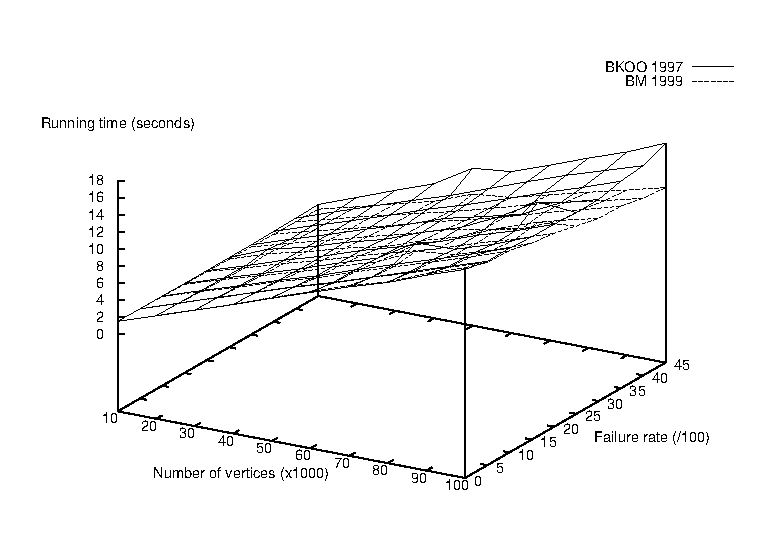
\includegraphics[height=\graphheight]{delaunay}}
\caption{Comparison of \bkoo\ and \bosemorin\ on Delaunay triangulations.}
\figlabel{delaunay}
\end{figure}

Figures~\ref{fig:mesh} and \ref{fig:graham} show similar results for
the case of regular quadrangle meshes and triangulations generated by
first sorting the points by $x$-coordinate and then using Graham's
scan (c.f., Ref.~[\cite{ps85}]) to triangulate the points.  Overall, these
results suggest that the \bosemorin\ algorithm not only performs better than
\bkoo\ in the worst case, but also in many practical cases.

\begin{figure}
\centerline{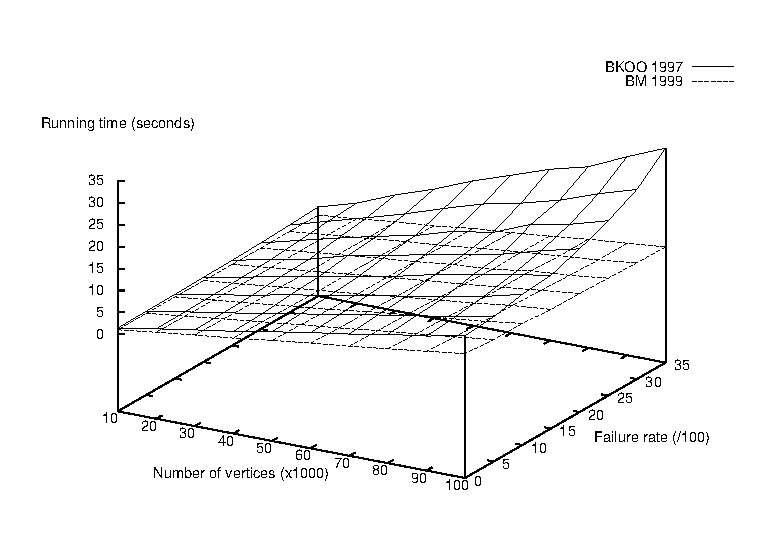
\includegraphics[height=\graphheight]{mesh}}
\caption{Comparison of \bkoo\ and \bosemorin\ on Meshes.}
\figlabel{mesh}
\end{figure}

\begin{figure}
\centerline{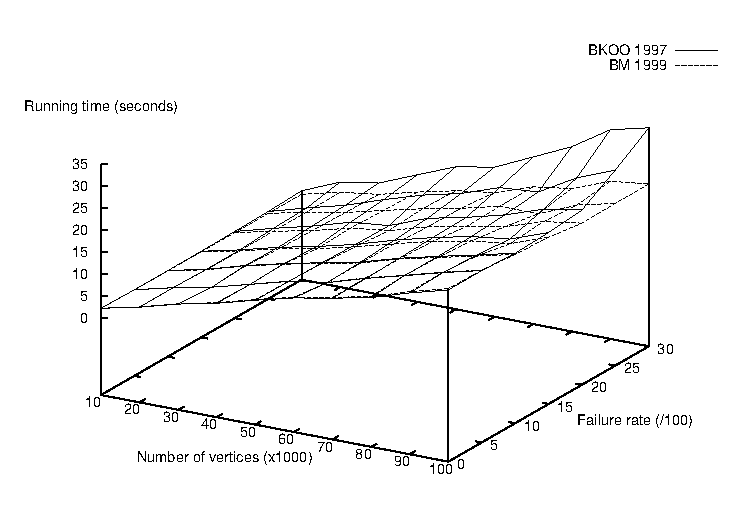
\includegraphics[height=\graphheight]{graham}}
\caption{Comparison of \bkoo\ and \bosemorin\ on Graham triangulations.}
\figlabel{graham}
\end{figure}


%%%%%%%%%%%%%%%%%%%%%%%%%%%%%%%%%%%%%%%%%%%%%%%%%%%%%%%%%%%%%%%%%%%%%%%%%
\section{Conclusions}\seclabel{conclusions}

We have shown how to traverse a connected planar subdivision with $n$
vertices using $O(1)$ additional memory and $O(n\log n)$ time.
\mbox{De Berg} \etal\cite{bkoo97} describe various extensions of
their algorithm, including curved subdivisions, window queries, and
traversing connected subsets of faces with a common attribute.  Our
modification of their algorithm results in improved running times for
all of these operations.  

An interesting theoretical open problem is to try and close the gap
between our $O(n\log n)$ upper bound for an $O(1)$ memory traversal
algorithm and the trivial $\Omega(n)$ lower bound.  Another
possibility is a tradeoff between running time and additional memory.
On the more practical side, we believe that a more careful
implementation of the $\preceq_p$ test could significantly reduce the
constants for the \bkoo\ and \bosemorin\ algorithms, making them more
competitive with algorithms that use mark bits.  In order to
encourage such research we have made our source code available on the
second author's web page (\url{http://www.cs.carleton.ca/~morin}).

\bibliography{traversal}
\bibliographystyle{unsrt}

\end{document}

